%% ------------------------------------------------------------------------- %%
\chapter{Conceitos}
\label{cap:conceitos}

\section{Computação em Nuvem}
\label{sec:computacao_nuvem}
Computação em nuvem é uma expressão utilizada para definir o fornecimento e uso de
insumos de computação como um serviço. Apesar do termo ainda não possuir uma
definição precisa, o conceito fundamental é que computação em nuvem pressupõe
um serviço\footnote{Neste momento, um serviço pode ser a alocação de
uma infraestrutura de servidores (\emph{Infrastructure as a Service} -- IaaS),
uma plataforma para desenvolver aplicações (\emph{Platform as a Service} -- 
PaaS) ou um \emph{software} pronto (\emph{Software as a Service} -- SaaS).}
elástico, virtualmente ilimitado e pago apenas pela porção realmente
utilizada, muito similar ao sistema de distribuição elétrica 
\cite{eecs:above-clouds}. Computação em nuvem tornou-se um negócio atrativo
a fornecedores e clientes graças ao barateamento de insumos necessários à
computação, como energia, poder de processamento, armazenamento e transmissão de
dados, permitindo uma economia de escala.

O objetivo final da computação em nuvem é prover um 
serviço ubíquo ao usuário, empresas ou pessoas físicas, que delegariam a gestão
dessa informação a terceiros competentes para prover um serviço de qualidade e 
seguro. Grandes empresas da área de tecnologia possuem soluções de computação em
nuvem, dentre as quais podemos citar Amazon \footnote{Amazon Elastic Compute
Cloud (Amazon EC2): \url{http://aws.amazon.com/pt/ec2/}}, Google
\footnote{Google Cloud Platform: \url{https://cloud.google.com/}}, Microsoft
\footnote{Windows Azure: \url{http://www.windowsazure.com/pt-br/}} e IBM
\footnote{IBM SmartCloud: \url{http://www.ibm.com/cloud-computing/us/en/}}.

Uma importante vantagem de \emph{cloud computing} é que com essa concentração de 
dados e serviços é possível desenvolver técnicas de otimização do uso de grandes
\emph{data centers}. Segundo estudo realizado por Barroso e Hölzle
\cite{barroso:case_energy_proportional} em 5000 servidores do Google, raramente
eles permanecem completamente ociosos e dificilmente operam próximos da sua
utilização máxima. Na maior parte do tempo estão trabalhando entre 10\% e 50\% 
do nível máximo. Os autores mostram que justamente nessa faixa de utilização
tais servidores são menos eficientes energeticamente.

Computação em nuvem é uma
candidata a ajudar a melhorar essa perspectiva. Através de virtualização e
reposicionamento automático de máquinas virtuais no data center,
uma funcionalidade disponível em produtos pagos como o VMware
vSphere \cite{vmware:vmotion} e softwares livres como o Xen 
\cite{alkmin:migracao_maquinas_virtuais}, é possível dimensionar
qual parcela do data center estará ativa em um dado momento dependendo da
demanda. Servidores com pouca utilização podem ser virtualizados em um único
servidor físico de modo que este trabalhe com uma utilização que seja mais
eficiente.

Vale ressaltar que em uma situação ideal, toda essa consolidação de servidores
é transparente ao usuário final. Em caso de um pico na demanda por um determinado
serviço, o provedor da nuvem deve garantir que haja uma resposta rápida da 
infraestrutura para suportar a nova carga requisitada. Dessa forma, são 
respeitados os acordos de nível de serviço (SLA - \emph{Service level agreement})
estabelecidos entre o usuário e o fornecedor da nuvem.

\section{Consumo Energético}
\label{sec:consumo_energetico}

Seguindo a tendência comentada na Seção \ref{sec:motivacao}, os serviços de TI
vem apresentando um forte crescimento devido à contínua migração de serviços,
análise de dados (\emph{Big Data}, \emph{Business Intelligence}, etc.) e
processamentos científicos para grandes data centers. Com isso, o consumo
energético total também tem aumentado. Em uma análise do custo
total de posse de um \emph{data center} de alta disponibilidade, cada \emph{rack}
\footnote{O autor define um \emph{rack} como um gabinete vazado de tamanho
padronizado (O mais comum é a versão de 19 polegadas de largura e 42 unidades
de altura. Cada unidade equivale a 1,75 polegada) e também gabinetes que contém
\emph{mainframes} e unidades de \emph{storage}.} possui um custo de US\$120.000
ao longo de 10 anos \cite{rasmussen:tco_data_center}.
Este custo está dividido conforme apresentado na Figura \ref{fig:tco_data_center}.

\newcommand{\slice}[4]{
  \pgfmathparse{0.5*#1+0.5*#2}
  \let\midangle\pgfmathresult

  % slice
  \draw[thick,fill=black!10] (0,0) -- (#1:1) arc (#1:#2:1) -- cycle;

  % outer label
  \node[label=\midangle:#4] at (\midangle:1) {};

  % inner label
  \pgfmathparse{min((#2-#1-10)/110*(-0.3),0)}
  \let\temp\pgfmathresult
  \pgfmathparse{max(\temp,-0.5) + 0.8}
  \let\innerpos\pgfmathresult
  \node at (\midangle:\innerpos) {#3};
}

\begin{figure}
\centering
\begin{tikzpicture}[scale=3]

\newcounter{a}
\newcounter{b}
\foreach \p/\t in {1/Monitoramento de Sistemas, 5/Gerenciamento de Projetos, 18/Equipamentos Elétricos,
                  6/Equipamentos de Refrigeração, 18/Engenharia e Instalações, 20/Eletricidade,
                   15/Serviços, 2/Rack, 15/Espaço}
  {
    \setcounter{a}{\value{b}}
    \addtocounter{b}{\p}
    \slice{\thea/100*360}
          {\theb/100*360}
          {\p\%}{\t}
  }
\end{tikzpicture}
\caption{Custo total de posse de um \emph{rack} em um \emph{data center} típico 
de alta disponibilidade \cite{rasmussen:tco_data_center}} \label{fig:tco_data_center}
\end{figure}

Como é possível ver na Figura \ref{fig:tco_data_center}, os custos relacionados
à eletricidade mais os gastos com equipamentos que apenas cumprem o propósito de
garantir que o servidor permaneça ligado e refrigerado totalizam 44\% 
(Eletricidade, Equipamentos de Refrigeração e Equipamentos Elétricos). Portanto,
uma redução nestes gastos gera um impacto tanto econômico quanto ambiental, com
a redução dos recursos naturais necessários para sustentar um \emph{data center}.

\subsection{Migração de Máquinas Virtuais}
Uma das grandes vantagens de manipular máquinas virtuais em um ambiente como
o de computação em nuvem é o fato de que é relativamente simples fazer uma 
realocação de máquinas virtuais de uma máquina hospedeira para outra, mesmo
enquanto a máquina virtual está funcionando \cite{vmware:vmotion}
\cite{alkmin:migracao_maquinas_virtuais}.

O objetivo desse processo é o de equalizar a infraestrutura utilizada
efetivamente com a demanda atual. Em momentos de poucas requisições é possível
minimizar o número de nós físicos que estão atendendo a carga de trabalho atual.
Enquanto isso, os nós ociosos ficam livres para serem
desligados ou colocados em algum estado de hibernação profunda, com baixo consumo
energético \cite{beloglazov:energy_efficient_allocation_virtual_machines}.
Quando há um aumento na demanda, é possível realizar o caminho inverso, 
distribuindo as máquinas virtuais em mais hospedeiros, garantindo o cumprimento
do SLA definido entre o provedor da nuvem e o usuário.

\subsection{Dimensionamento Dinâmico de Tensão e Frequência}
\label{subsec:dvfs}
A estratégia de dimensionamento dinâmico de tensão e frequência, do inglês 
\emph{dynamic voltage and frequency scaling}, é uma tática 
bastante difundida entre os fabricantes de processadores como uma forma pouco
invasiva de economizar energia elétrica. Tecnologias como o Intel Speed Step
e o AMD Coll'n'Quiet ajustam automaticamente em hardware a tensão
e frequência dos processadores proporcionalmente com suas cargas de trabalho
atuais \cite{lago:escalonamento_com_prioridade_eficiente}.


\section{Escalonamento de Tarefas}
\label{sec:escalonamento_tarefas}
Segundo \cite{lago:escalonamento_com_prioridade_eficiente}, o escalonamento de 
tarefas pode ser visto através de duas óticas: a do usuário da nuvem, que deseja
que sua tarefa execute o mais rapidamente possível e com o menor custo e a 
perspectiva do provedor da nuvem, interessado em reduzir os recursos utilizados,
gerando economias na manutenção e energia elétrica. Esta monografia foca no
escalonamento pelo ponto de vista do provedor. 


\subsection{\emph{Heterogeneous Earliest Finish Time}}
\label{subsec:heft}
O algoritmo \emph{Heterogeneous Earliest Finish Time} -- HEFT é um algoritmo de
escalonamento de fluxos de trabalho modelados utilizando um digrafo acíclico
(\emph{Directed acyclic graph} -- DAG) para um número limitado de computadores
heterogêneos \cite{kim:virtual_computing}.

O HEFT é um exemplo de escalonador \emph{baseado em lista}. Ou seja, funciona
ordenando as tarefas a serem executadas ao definir prioridades de escalonamento.
Em seguida, processa uma tarefa por vez até que um escalonamento válido seja
produzido. Para cada tarefa, é definido o processador que irá acomodar esta
tarefa. Todo o processamento do HEFT é feito antes do escalonamento ser
executado, ou seja, é um escalonador \emph{off-line}.

Como o problema de escalonamento de
tarefas é NP-difícil, o HEFT é frequentemente utilizado como
referência na literatura para comparar o desempenho de novas propostas, 
como por exemplo em \cite{batista:embedding_software_requirements}.

O HEFT recebe como entrada um conjunto de tarefas modeladas como um DAG, um
conjunto de nós computacionais, os tempos para executar uma tarefa em um dado nó
e os tempos necessários para comunicar os resultados de uma tarefa para cada uma
de suas tarefas filhas no DAG. Como saída o algoritmo gera um escalonamento,
mapeando cada tarefa a uma máquina.

O HEFT consiste de duas fases principais:

\begin{description}
	\item[Fase de priorização] Cálculo da prioridade das tarefas e criação
		da lista de escalonamento com base neste cálculo
	\item[Fase de seleção] Mapeamento de cada tarefa em uma máquina para
		processamento
\end{description}

\subsubsection{Fase de Priorização}
Nesta fase do algoritmo HEFT, cada tarefa deve ser priorizada considerando
o comprimento do caminho crítico (Ou seja, o maior caminho) de uma dada tarefa
até a tarefa final no fluxo de trabalho. (Passos 1 a 5 no algoritmo 
\proc{Heterogeneous-Earliest-Finish-Time}). A lista de tarefas a serem
executadas é então ordenada pela ordem decrescente do comprimento do caminho
crítico, com empates sendo decididos aleatoriamente.
Com essa ordem, é produzida uma ordenação topológica das tarefas, 
preservando as restrições de precedência do DAG.

A prioridade de uma tarefa $n_i$ é definida recursivamente como:

$$ \label{eq:rank} rank_u(n_i) = \overline{w_i} + \max_{n_j \in succ(n_i)} (\overline{c_{i,j}} + rank_u(n_j)) $$

onde $n_i$ representa a $i$-ésima tarefa, $\overline{w_i}$ é uma média do custo
computacional em uma unidade de tempo da tarefa $i$ entre todos os
processadores, $succ(n_i)$ é o conjunto de todas as tarefas que dependem
imediatamente da tarefa $n_i$ e $\overline{c_{i,j}}$ é o custo de comunicação
dos dados transferidos entre as tarefas $n_i$ e $n_j$ na mesma unidade de tempo
utilizada antes. %TODO ver no artigo original do HEFT

Note que o cálculo de $rank_u(n_i)$ depende do cálculo do $rank_u$ de todas as
suas tarefas filhas. A noção intuitiva por trás do $rank_u$ é que ele deve
representar a distância esperada de qualquer tarefa até o fim da execução do
\emph{workflow}.

Ao processar primeiramente as tarefas que estão em um potencial caminho crítico
do DAG, o HEFT possui à sua disposição máquinas mais poderosas disponíveis para
o processamento. Desta forma, pode aplicá-las para garantir que este caminho
crítico seja processado o mais rápido possível. Um caminho crítico é definido
como uma sequência de vértices conectados cujo tempo de execução é o limitante
inferior no tempo total de execução do fluxo de trabalho

\begin{codebox}
\Procname{$\proc{Heterogeneous-Earliest-Finish-Time}()$}
\li	Defina os custos computacionais das tarefas e os custos de comunicação entre as tarefas
\zi com valores médios
\li	Calcule $rank_u$ para todas as tarefas varrendo o grafo de ``baixo para cima'',
	iniciando \\pela tarefa final.
\li Ordene as tarefas em uma lista de escalonamento utilizando uma ordem não
\zi crescente de valores de $rank_u$.
\li 	\While há tarefas não escalonadas na lista
\li 		\Do
				Selecione a primeira tarefa, $n_i$ da lista de escalonamento.
\li				\For cada processador $p_k$ no conjunto de processadores $(p_k \in P)$
\li 				\Do
						Calcule o tempo mais cedo de conclusão da tarefa  $n_i$,
						considerando que ela execute 
\zi         em $p_k$
					\End
\li				Defina a tarefa $n_i$ para executar no processador $p_j$ que
					minimiza o tempo mais
\zi       cedo de conclusão da tarefa $n_i$.
			\End
\End
\end{codebox}

\subsubsection{Fase de Seleção}
Na maioria dos algoritmos de escalonamento, o tempo mais cedo de
conclusão (\emph{earliest finish time} -- EFT) de um dado
processador $p_j$ para a execução de uma tarefa é o momento quando
$p_j$ completa a execução da última tarefa que foi designada a
ele. No entanto, o algoritmo HEFT possui uma política de inserção
que considera a possibilidade de inserir uma tarefa em um espaço
vago entre duas tarefas já escalonadas em um processador
\cite{topcoglu:heft}.
%O comprimento de um intervalo de tempo vago, ou seja, 
%a diferença entre o tempo de início e término de duas tarefas
%que já foram escalonadas em um mesmo processador, deve ser
%maior ou igual ao tempo necessário para a computação da tarefa,
%possivelmente descontado o tempo de comunicação entre
%processadores.
Note que o escalonamento neste intervalo deve obedecer às
restrições de precedência.

No algoritmo HEFT, a busca por um \emph{slot} de tempo vago
para uma tarefa $n_i$ em um processador $p_j$ começa no
momento igual ao tempo que a tarefa $n_i$ estará pronta para
executar em $p_j$, ou seja, o momento quando todos os dados
de entrada de $n_i$ foram enviados pelos predecessores imediatos
de $n_i$ ao processador $p_j$. A busca continua até que seja
encontrado um intervalo de tempo capaz de suportar o custo
computacional de $n_i$ \cite{topcoglu:heft}.


\subsubsection{Análise de Complexidade do HEFT}
No algoritmo \proc{Heterogeneous-Earliest-Finish-Time}, o passo 1 toma tempo
$O(e \times p)$ para computar as médias enquanto o passo 2 toma tempo $O(e)$ para 
computar o comprimento do caminho crítico, onde $e$ é o número de arestas no 
DAG e $p$ o número de processadores. Para $n$ tarefas a serem escalonadas, 
o passo 3 necessita de um tempo $O(n \log n)$ para ordenar as tarefas pelo
comprimento de seus caminhos críticos. Seja $a$ o número de tarefas que tem
$n_i$ como predecessora no DAG, então os passos 5-8 ocupam um tempo
$O(a \times p)$ para uma tarefa $n_i$, assim, o laço enquanto necessita de um 
tempo $O(e \times p)$. Portanto, a complexidade do algoritmo HEFT é  $O(e
\times p)$.

\subsubsection{Exemplo de Execução}
\begin{figure}[ht]
\centering
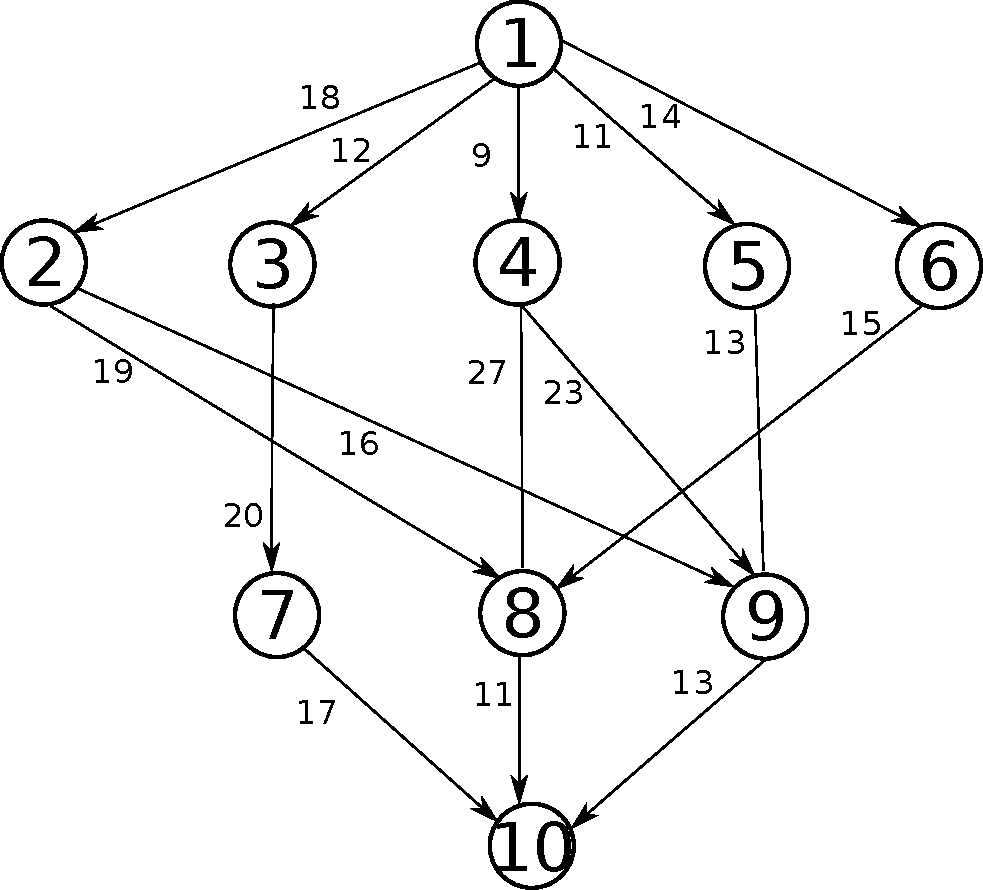
\includegraphics[width=0.5\linewidth]{dag_heft.pdf}
\caption{Fluxo de trabalho simulado, contendo os custos médios de
transmissão de dados entre um nó de processamento e outro}
\label{fig:dag_heft}
\end{figure}

Para uma execução simulada do algoritmo HEFT, consideramos o fluxo de trabalho
apresentado no artigo original do algoritmo, \cite{topcoglu:heft}, descrito na
Figura \ref{fig:dag_heft}. Cada vértice do DAG é uma tarefa a ser executada em
um dos três processadores (heterogêneos) disponíveis: P1, P2 e P3. Os rótulos
nas arestas indicam o tempo necessário para transferir os resultados de uma
tarefa entre dois processadores \emph{distintos}.

Para uma dada tarefa, o tempo para processá-la em cada um dos processadores está
descrito na Tabela \ref{tab:custos_computacionais}. Com os valores apresentados
é possível calcular o valor de $rank_u$, seguindo a fórmula apresentada
anteriormente. O resultado está também na Tabela
\ref{tab:custos_computacionais}. O escalonamento resultante da execução do HEFT
com o grafo da Figura \ref{fig:dag_heft} está apresentado na Figura
\ref{fig:escalonamento_heft}. Note que o tempo total de execução do fluxo de
trabalho após o escalonamento feito pelo HEFT é de 80 segundos no total. Em
comparação, se todas as tarefas fossem processadas na máquina P1 o tempo de
execução seria de 127 segundos, na máquina P2 de 130 segundos e na máquina P3 de
143 segundos. Isso confere ao HEFT ganhos de 37\%, 38,5\% e 44\%
respectivamente.

\begin{figure}[ht]
\centering
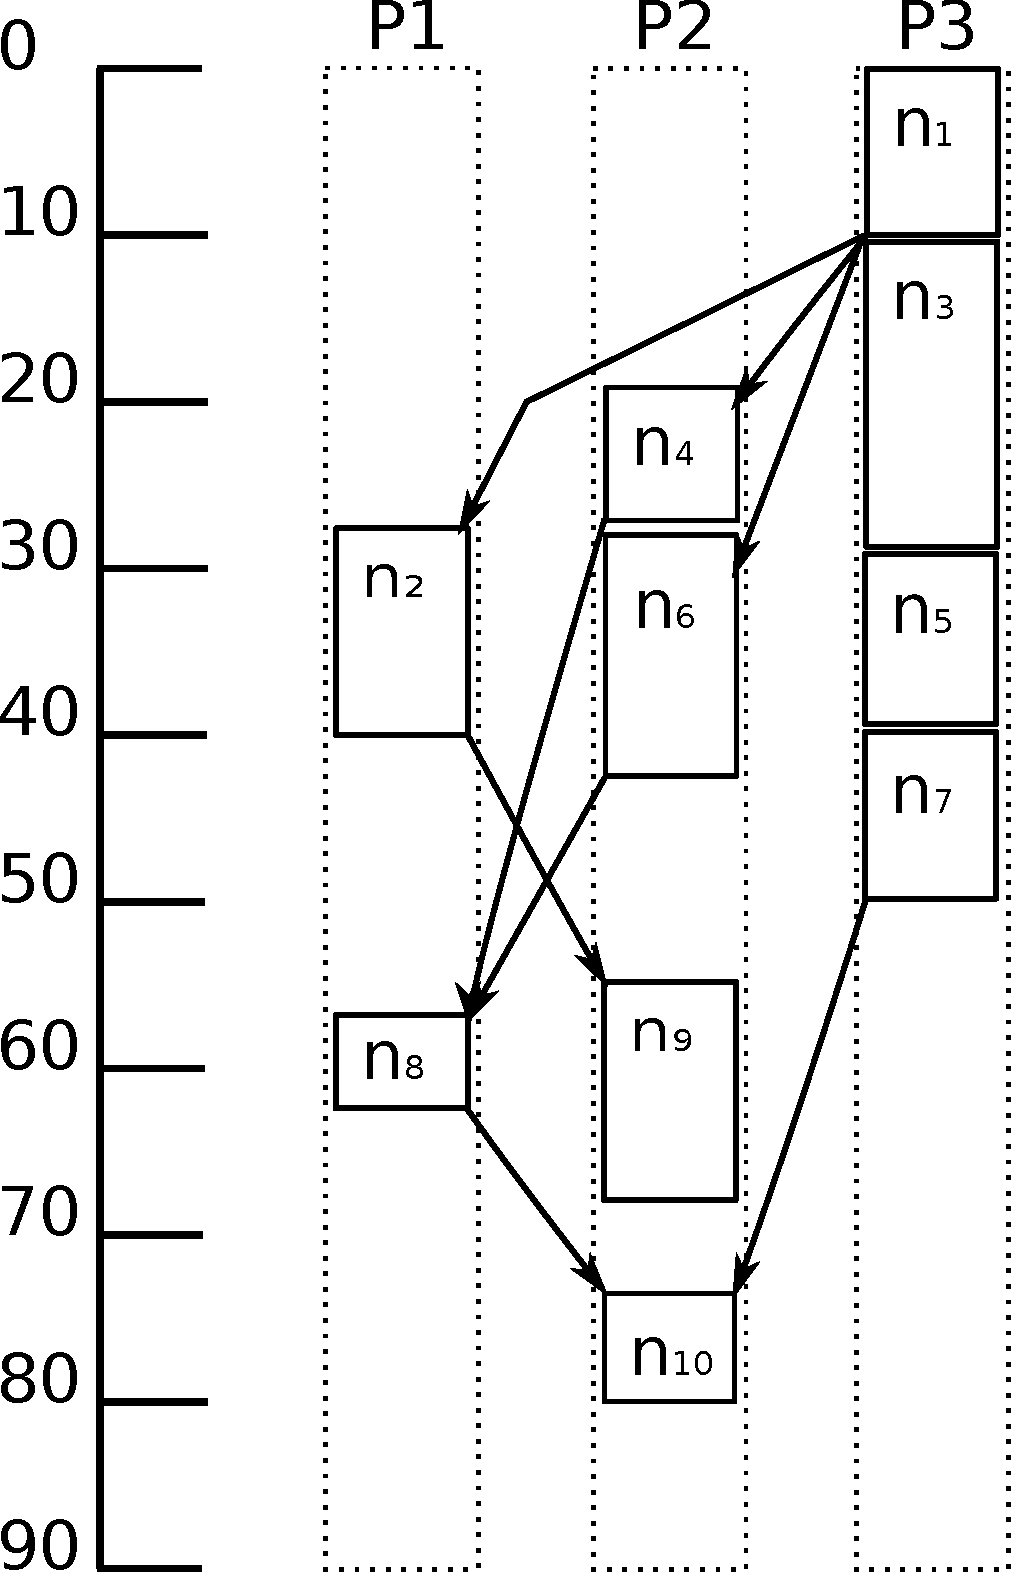
\includegraphics[width=0.3\linewidth]{escalonamento_heft.pdf}
\caption{Escalonamento produzido pelo algoritmo HEFT}
\label{fig:escalonamento_heft}
\end{figure}


\begin{table}[ht]
	\centering
    \begin{tabular}{|c|c|c|c|c|}
    \hline
    \textbf{Tarefa} & \textbf{P1 (s)} & \textbf{P2 (s)} & \textbf{P3 (s)} & $rank_u(n_i)$ \\ \hline
	1               & 14          & 16          & 9           & 108.000       \\
	2               & 13          & 19          & 18          & 77.000        \\
	3               & 11          & 13          & 19          & 80.000        \\
	4               & 13          & 8           & 17          & 80.000        \\
	5               & 12          & 13          & 10          & 69.000        \\
	6               & 13          & 16          & 9           & 63.333        \\
	7               & 7           & 15          & 11          & 42.667        \\
	8               & 5           & 11          & 14          & 35.667        \\
	9               & 18          & 12          & 20          & 44.333        \\
	10              & 21          & 7           & 16          & 14.667        \\ \hline
    \end{tabular}
    \caption {Custos computacionais de uma tarefa em um dado
    computador}
    \label{tab:custos_computacionais}
\end{table}


\subsection{Embutindo Requisitos de Software no Escalonamento}
Notamos neste momento que tarefas a serem executadas em um ambiente de
computação em nuvem ou em grade podem requisitar algum software específico para
sua execução. Em \cite{batista:embedding_software_requirements} é apresentada
uma técnica a ser descrita nesta seção para modificar o DAG de dependências
entre as tarefas a fim de incorporar tais requisitos de software.

Trivialmente há duas possibilidades para resolver o problema: a primeira
possibilidade é alocar apenas uma máquina virtual para cada software distinto a
ser executado no fluxo de trabalho. Esta ideia tem o problema de gerar falsas
dependências entre as tarefas, já que apenas uma tarefa pode executar por vez 
em uma máquina e, assim, processos computacionais que poderiam executar em 
paralelo passam a ter que ser processadas sequencialmente. Outra alternativa é
alocar uma máquina virtual para cada tarefa. Esta abordagem além de ser custosa 
em recursos alocados não necessariamente garante o menor tempo de execução
possível pois o tráfego de rede entre os nós de processamento pode não ser o
ótimo.

Há uma quantidade exponencial de diferentes formas de alocar máquinas para 
executar um dado fluxo de trabalho. Esse número vem do fato que alocar tarefas
em máquinas é equivalente a encontrar o número de partições de um conjunto, 
modelado pelo número de Bell, conforme visto nas equações \ref{eq:numero_bell_1}
e \ref{eq:numero_bell_2}. O número de Bell é definido como uma recorrência,
com $B_n$ sendo o número de partições de um conjunto de tamanho $n$.
Assim, os autores apresentam uma heurística para o problema.

\begin{align} \label{eq:numero_bell_1}
	B_0 &= 1\\ \label{eq:numero_bell_2}
	B_{n+1} &= \sum_{k=0}^{n}{{n \choose k}B_k}
\end{align}

O objetivo da heurística proposta é reduzir o tráfego de rede necessário e, 
ao mesmo tempo, evitar aumentar o caminho crítico dos fluxos de trabalho.
Isto é feito através da busca das tarefas que possuem os mesmos requisitos de
software em um dado caminho do DAG. Dessa forma, há a instanciação de apenas uma
VM para cada dependência de software em um caminho.

%\begin{codebox}
%\Procname{$\proc{Modificador de DAG}(\mathcal{D})$}
%\li \Comment \textbf{Entrada:} Um DAG $\mathcal{D}$ com requisitos de software 
%	$\mathcal{S}$ ainda não embutidos no DAG.
%
%\li \Comment \textbf{Saída:} Um DAG $\mathcal{M}$ com os requisitos de software embutidos.
%\li \For cada caminho $h \in \mathcal{D}$
%		\Do
%\li			\For cada tarefa $t \in h$
%\li				\Do
%					Inclua $t$ no conjunto $P_{h,s}$, onde $S_s$ é a dependência de software de $t$
%				\End
%		\End
%\li	Crie uma nova tarefa $R$ com peso 0
%\li 	\While há pelo menos um conjunto $P$
%\li 		\Do
%				\For cada software $s \in \mathcal{S} | \exists$ pelo menos um conjunto $P_{h,s}$
%\li 				\Do
%						Faça $P_\begin{savenotes}
%					\End
%\li				Defina a tarefa $n_i$ para executar no processador $p_j$ que
%				minimiza o\\ Earliest	Execution Finish Time da tarefa $n_i$.
%			\End
%\End
%\end{codebox}


\section{Simuladores de computação em nuvem e fluxos de trabalho}
\label{sec:ambiente_simulacao}
Uma vez concebidos novos algoritmos ou abordagens para problemas em computação
em nuvem há algumas maneiras de realizar experimentos para estudar o desempenho
de tais mudanças: uma possibilidade seria a execução de instâncias
reais dos problemas em provedores reais de \emph{cloud computing}. Essa alternativa
possui como problema o custo monetário envolvido na instanciação de máquinas
virtuais por um tempo prolongado. Ainda, não há o controle sobre o ambiente 
de simulação, prejudicando a reproducibilidade dos experimentos. Outra opção
seria a de instalar um ambiente próprio para experimentos, novamente esbarrando
em problemas financeiros. 

Uma alternativa mais factível é a utilização de ambientes de simulação computacional.
Estas ferramentas abrem a possibilidade de avaliar uma hipótese em um ambiente
totalmente controlado e facilmente reproduzível. Ainda, há um ganho na facilidade
de simular diferentes variações de ambientes, facilitando a busca por gargalos
na eficiência dos algoritmos utilizados. Esses benefícios vem ao custo da
simplificação dos modelos utilizados para simular o ambiente proposto.

Nesta seção serão apresentados os principais simuladores utilizados nos 
experimentos descritos no Capítulo \ref{cap:experimentos}: CloudSim, WorkflowSim
e PowerWorkflowSim.

\subsection{CloudSim}

CloudSim \cite{calheiros:cloudsim} é um simulador para computação em nuvem,
reconhecido academicamente com citações em mais de 300 trabalhos indexados pelo
Google Scholar \cite{google:cloudsim}. Ele provê as funcionalidades de simulação
de máquinas virtuais, \emph{hosts}, \emph{data centers}, políticas de
provisionamento de recursos, tarefas a serem executadas em máquinas virtuais
(\emph{cloudlets}) além de efetuar análises de duração de simulações e consumo
de energia. Ainda, é software livre, disponibilizado sob a licença GNU LGPL
\cite{cloudsim:site}. Na Figura \ref{fig:arquitetura_cloudsim} é possível ver a
arquitetura projetada pelos desenvolvedores do CloudSim já a Figura
\ref{fig:classes_cloudsim} apresenta o diagrama de classes da implmentação do
CloudSim.

\begin{figure}[ht]
\centering
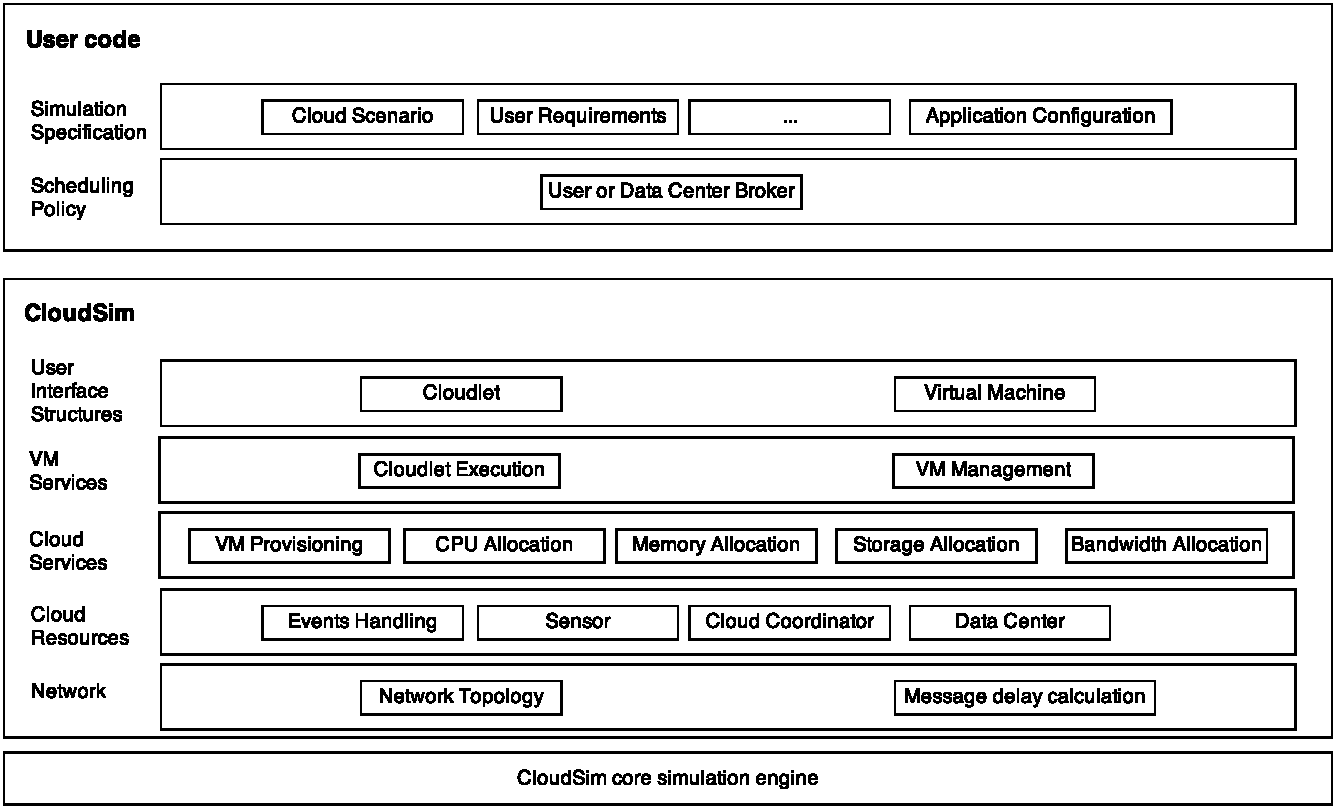
\includegraphics[width=\linewidth]{CloudSim.pdf}
\caption{Arquitetura do CloudSim, adaptada de \cite{calheiros:cloudsim}}
\label{fig:arquitetura_cloudsim}
\end{figure}

\begin{figure}[ht]
\centering
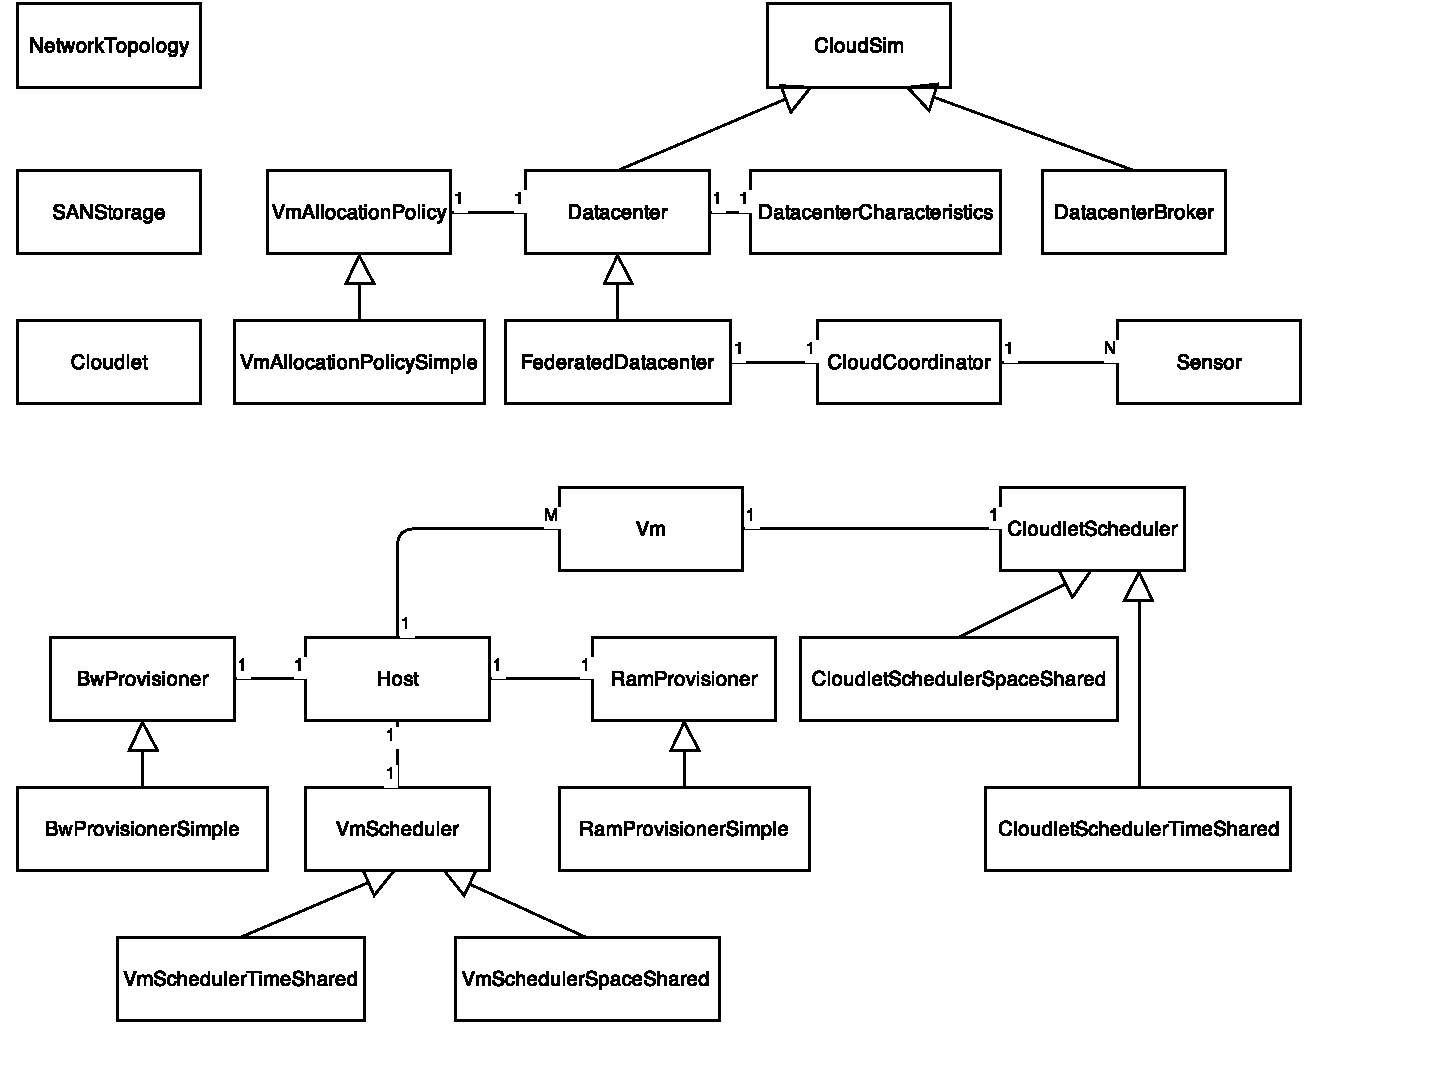
\includegraphics[width=\linewidth]{ClassesCloudSim.pdf}
\caption{Diagrama de classes simplificado do CloudSim, adaptada de \cite{calheiros:cloudsim}}
\label{fig:classes_cloudsim}
\end{figure}

A arquitetura em camadas do CloudSim permite uma separação clara das diferentes
possibilidades de extensão e experimentação em um ambiente de computação em nuvem.
Por exemplo, todo o código responsável pela simulação energética do CloudSim
é na verdade uma especialização das classes originais do simulador. Assim,
a classe \ttt{PowerDatacenter} e \ttt{PowerHost} são classes herdadas de
\ttt{Datacenter} e \ttt{Host} respectivamente.

Com a boa aceitação do CloudSim como uma ferramenta de simulação, passaram a 
surgir simuladores mais especializados, como por exemplo o WorkflowSim, assunto
da Seção \ref{subsec:workflowsim}.

\subsubsection{Modelagem de uma Nuvem Computacional}

Os serviços de infraestrutura providos por nuvens podem ser simulados através 
da extensão da classe \ttt{Datacenter} do CloudSim. Esta entidade gerencia
diversos \ttt{Host}s. Cada \ttt{Host} possui uma capacidade de processamento 
pré determinada, medida em milhões de instruções por segundo (MIPS) e podendo 
ser com apenas um único ou vários núcleos de processamento, memória e
armazenamento. Um \ttt{Host} pode incorporar uma ou mais \ttt{Vm} (Máquina virtual)
de acordo com as políticas de alocação definidas nele pelo administrador da nuvem.
Uma política de alocação é definida como as operações relacionadas a uma
\ttt{Vm} durante seu ciclo de vida: escolha de um \ttt{Host}, criação, 
migração e destruição.

De maneira similar, cada \ttt{Vm} possui capacidades de processamento, memória,
largura de banda e número de processadores definidos no momento da sua criação.
Ainda, pode executar uma ou mais tarefas, \ttt{Cloudlet}s, obedecendo-se as
políticas de provisionamento de aplicações.

\subsubsection{Modelagem do Consumo Energético}
Como discutido anteriormente, o CloudSim possui uma extensão que incorpora 
a modelagem do consumo energético das máquinas utilizadas na simulação. Nessa 
extensão cada elemento de processamento (Tipicamente um núcleo) inclui um
objeto que estende o tipo abstrato \ttt{PowerModel}, responsável por gerenciar o
consumo energético. Isso garante um desacoplamento entre o processamento e 
a estratégia de modelagem energética empregadas. Por exemplo,
um PowerModel pode levar em conta a estratégia de DVFS descrita na Seção 
\ref{subsec:dvfs} enquanto outro não. O CloudSim apresenta algumas implementações
concretas da classe \ttt{PowerModel}. A técnica de modelagem empregada é descrita
em \cite{beloglazov:cloudsim_power}.


\subsection{WorkflowSim}
\label{subsec:workflowsim}
Apesar de ser bem consolidado como ferramenta de simulação de computação em nuvem,
o CloudSim não possui certas características necessárias à simulação de 
\emph{workflows} científicos como por exemplo as ineficiências causadas pelo
uso de sistemas heterogêneos e falhas. Ainda, percebe-se a falta de suporte a 
técnicas de otimização de execução de \emph{workflows} amplamente utilizadas
tais como o \emph{clustering} de tarefas. De forma a resolver essas demandas
o WorkflowSim foi criado tendo como base o CloudSim \cite{chen:workflowsim}.
A licença do WorkflowSim foi levemente alterada, sua licença é a Globus Toolkit
Public License\footnote{Informações sobre a licença disponíveis em 
\url{http://www.globus.org/toolkit/download/license.html}}
\cite{workflowsim:license}.

Enquanto o CloudSim se concentra na execução de uma única carga de trabalho,
o WorkflowSim foca no escalonamento do \emph{workflow} e sua execução. O último
processa \emph{workflows} modelados como DAGs, realizando um escalonamento que 
obedece a precedência imposta pelo DAG. Ainda, é possível implementar diferentes
algoritmos de escalonamento para avaliar suas eficiências. Uma das atividades desse
TCC foi implementar o algoritmo HEFT comentado na Seção \ref{subsec:heft} no 
WorkflowSim. \footnote{Outros algoritmos de escalonamento tais como FCFS, 
MinMin, MaxMin, MCT e \emph{Data aware} já estão implementados na versão atual
(1.0)}

\begin{figure}[ht]
\centering
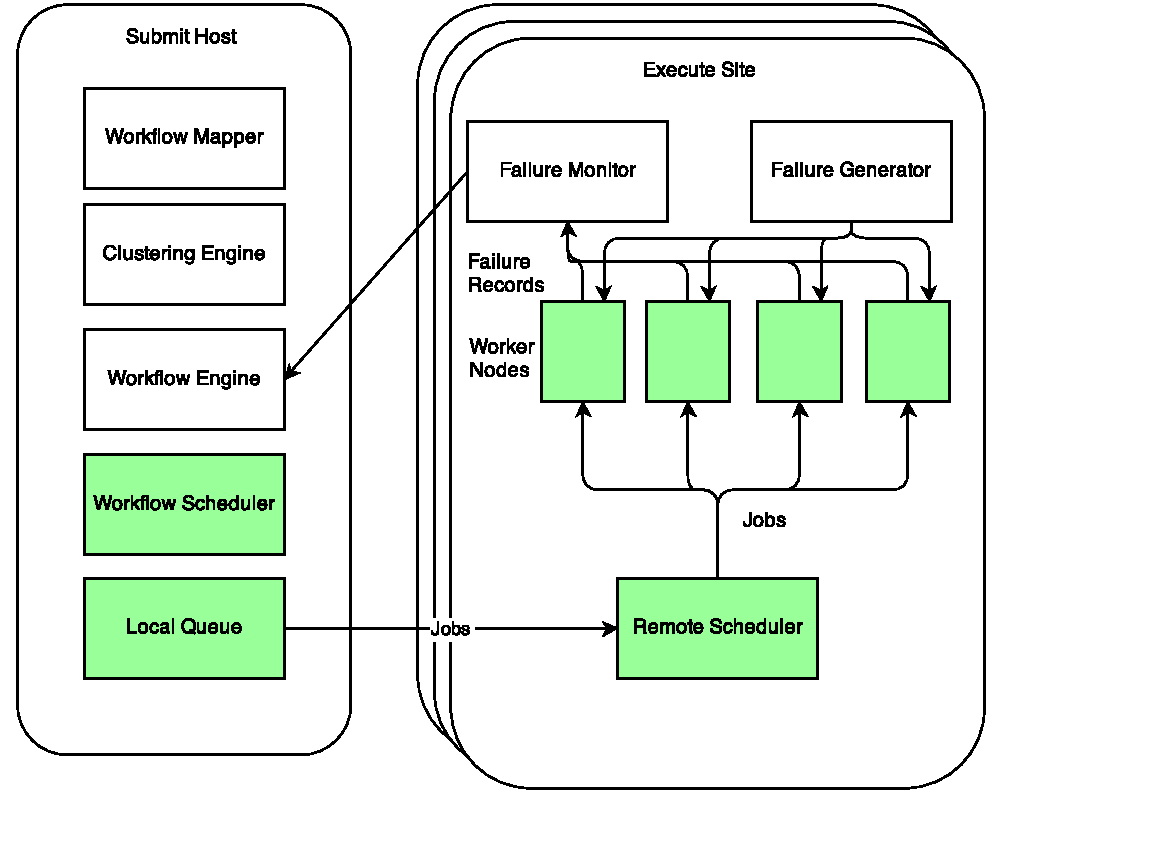
\includegraphics[width=10cm]{WorkflowSim.pdf}
\caption{Arquitetura do WorkflowSim, adaptado de \cite{chen:workflowsim}.
Os componentes em verde são providos pelo CloudSim}
\label{fig:arquitetura_workflowsim}
\end{figure}

Como é possível ver na Figura \ref{fig:arquitetura_workflowsim}, há múltiplas
camadas de componentes envolvidos na preparação e execução do \emph{workflow}:
Um \ttt{Workflow Mapper} que mapeia \emph{workflows} abstratos em
\emph{workflows} concretos, dependentes do local de execução; uma \ttt{Workflow
Engine} que gerencia a dependência de dados e um \ttt{Workflow Scheduler} para
associar tarefas aos processadores, por fim a \ttt{Clustering Engine} é
responsável por agrupar tarefas menores em um pacote maior.


\subsection{CloudSim\_DVFS}
\label{subsec:cloudsim_dvfs}

Um segundo simulador baseado no CloudSim foi desenvolvido de maneira
concomitante com o WorkflowSim. O CloudSim\_DVFS foi lançado em outubro de 2013
no artigo \cite{guerout:energy_aware_simulation}. Esta ferramenta também
implementa  o processamento de fluxos de trabalho modelados como DAGs e
descritos utilizando o mesmo formato de entrada que o WorkflowSim: Arquivos XML
no formato DAX definido pelo projeto Pegasus \cite{pegasus:dax}.

A principal diferença do CloudSim\_DVFS para o simulador anterior é o foco em
simulações energéticas, como já reflete seu nome. Ele aprofunda a API de
simulação energética disponível no CloudSim. Agora, são definidas diferentes
estratégias de DVFS:

\begin{description}
  \item[Performance] Utiliza a CPU em frequência máxima (Sem DVFS)
  \item[PowerSave] Utiliza a CPU na frequência mínima
  \item[UserSpace] Permite que o usuário defina a faixa de frequência que
    a máquina deve operar
  \item[Conservative] Utiliza um limite superior e um inferior para decidir
    as mudanças na frequência da CPU. Caso a carga esteja acima do limite
    superior, a frequência é aumentada se possível. Caso ela esteja abaixo
    do limite inferior tenta diminuir a frequência.
\end{description}

\subsubsection{Modelagem energética} % (fold)
\label{ssub:modelagem_energ_tica}

Os autores do CloudSim\_DVFS optaram pela estratégia ``caixa-preta'' para a
modelagem do consumo energético de uma máquina. Desta forma, é capaz de abstrair
detalhes da construção dos processadores atuais e trabalhar em um modelo de
alto nível. O modelo descreve dois valores de consumo energético para cada
faixa de frequência disponível às estratégias de DVFS: consumo em máxima
capacidade (100\% da faixa escolhida) e quando a máquina está ociosa (0\% 
da faixa escolhida). Por fim, é feita uma interpolação linear entre estes
dois níveis, com base na proporção de tempo que a máquina esteve realizando
processamento. A fórmula utilizada está descrita na equação \ref{eq:modelagem_energetica}. $\alpha$ é o uso de CPU e $P_{CPUIdle}$ e $P_{CPUFull}$ são os valores
de potência consumida pela CPU com 0\% e 100\% de utilização respectivamente.

\begin{equation}
P_{TOT} = (1 - \alpha)P_{CPUIdle} + (\alpha)P_{CPUFull} \label{eq:modelagem_energetica}  
\end{equation}

\begin{table}
    \centering
    \begin{tabular}{c|cllll}
    \hline
    \textbf{Velocidades (GHz)} & \textbf{0.8} & \textbf{1.0} & \textbf{1.2} & \textbf{1.5} & \textbf{1.7} \\ \hline
    \textbf{Nível ocioso (W)}       & 140          & 146          & 153          & 159          & 167          \\
    \textbf{Nível máximo (W)}  & 228          & 238          & 249          & 260          & 272          \\ \hline
    \end{tabular}
    \caption{Frequências do Grid'5000 Reims com as medidas de potência durante
    cargas mínima e máxima (0\% e 100\% de uso dos 24 núcleos de um nó de processamento)
    \cite{guerout:energy_aware_simulation}}
\end{table}


% subsubsection modelagem_energ_tica (end)